\chapter{Experimental Results} \label{chap:results}

\section{Experiment setup}
\subsection{Datasets}

In order to validate the experimental methods discussed in this thesis, various datasets we utilized as shown in Table \ref{table:expData}. 


\begin{table}[ht]
\caption{Summary of experimental datasets} % title of Table
\centering % used for centering table
\begin{tabular}{l l l l l l} % centered columns (4 columns)
\hline %inserts single horizontal lines
Bimodal dataset & Method & Samples & Classes & Learning task & Feature type \\ %[0.5ex] % inserts table
%heading
\hline % inserts single horizontal line
RNA-seq + miRNA-seq & SDAE & 3988 & 9 & classification & real\\ 
RNA-seq + miRNA-seq & DCF & 3988 & 9 & classification & real\\ 
RNA-seq + miRNA-seq & DE & 3988 & 9 & classification & real\\ 
CNV + RNA-seq & DCF & 3988 & 9 & classification & real\\ 
CNV + RNA-seq & SDAE & 3988 & 9 & classification & real\\ 
miRNA-seq + SNV & DCF & 3375 & 6 & classification & real + integer\\ miRNA-seq + SNV & SDAE & 3375 & 6 & classification & real + integer\\ 
%Exp7 & dp & fet & - & regression     & real\\ 
[1ex]   % [1ex] adds vertical space 
\hline %inserts single line
\end{tabular}
\label{table:expData}
\end{table}

\section{Results}

In the following, we report the results from all experiments. In all cases, experiments were constructed using the following experimental settings and constraints:

\begin{itemize}
    \item The datasets were divided into a 60/20/20 split for training, validation, and testing, respectively.
    \item Hyperparameter tuning was performed on the cross validation set.
    \item Experiments were repeated 10 times using 10 fold cross validation on the training set.
\end{itemize}

\subsection{miRNA-seq + RNA-seq}\label{subsub:m_r_SDAE}

\subsubsection{SDAE}

\begin{figure}[H]
     \centering
     \begin{subfigure}[b]{0.49\textwidth}
         \centering
         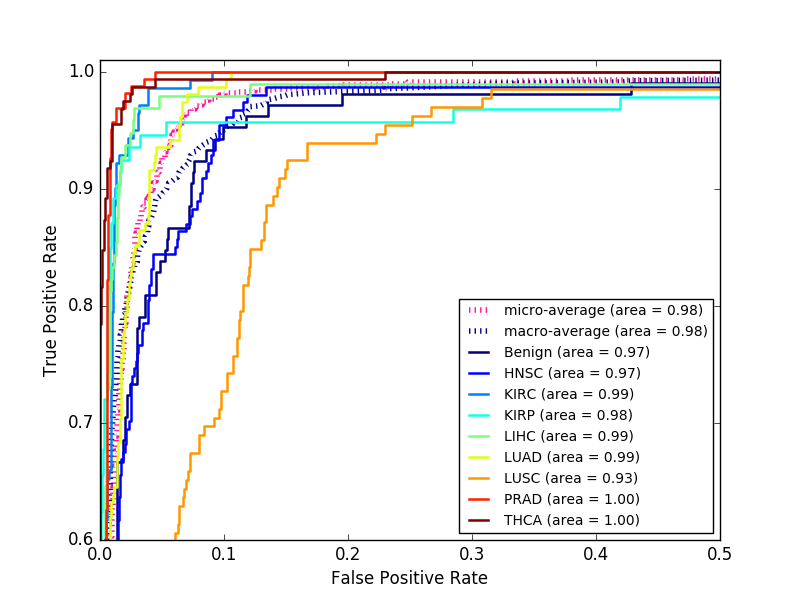
\includegraphics[width=\textwidth]{img/m_r/m_r_sdae_dgmu_roc.png}
         \caption{}
     \end{subfigure}
     \hfill
     \begin{subfigure}[b]{0.49\textwidth}
         \centering
         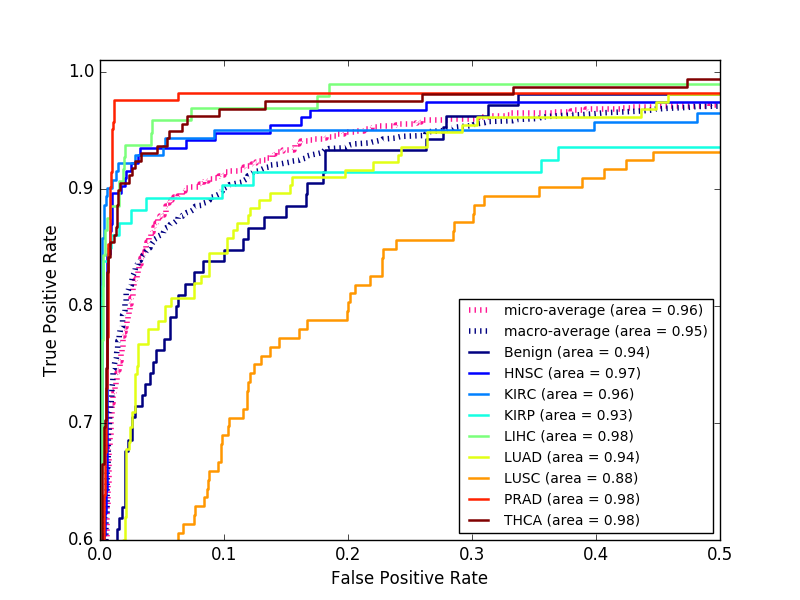
\includegraphics[width=\textwidth]{img/m_r/m_r_sdae_gmu_roc.png}
         \caption{}
     \end{subfigure}
     \hfill
     \begin{subfigure}[b]{0.49\textwidth}
         \centering
         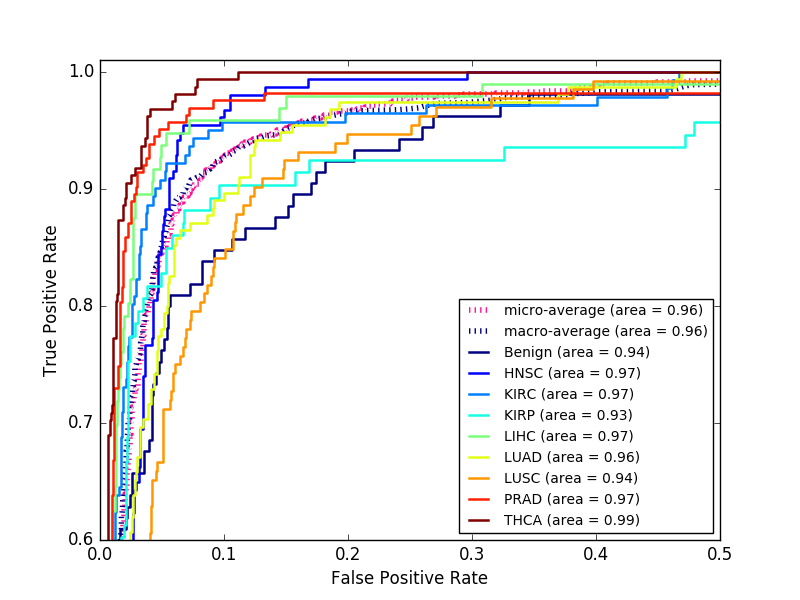
\includegraphics[width=\textwidth]{img/m_r/m_r_sdae_mlp_roc.png}
         \caption{}
     \end{subfigure}
     \begin{subfigure}[b]{0.49\textwidth}
         \centering
         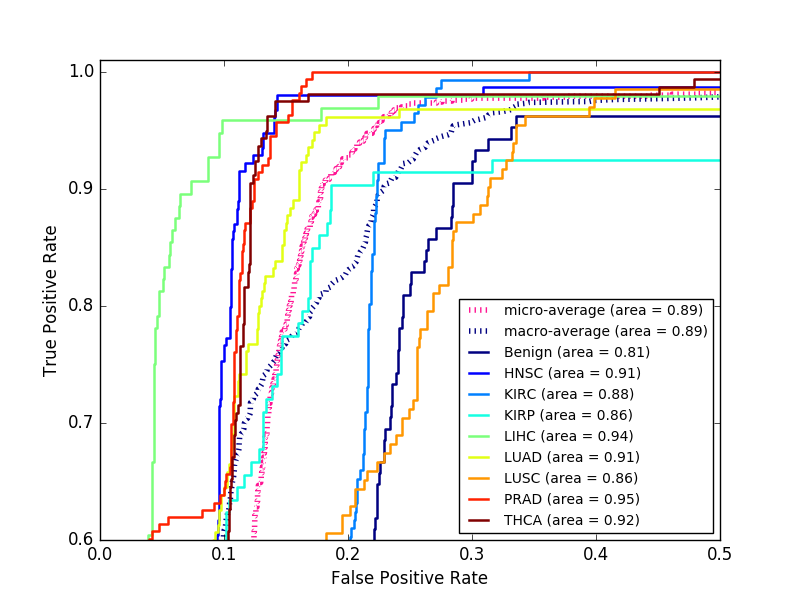
\includegraphics[width=\textwidth]{img/m_r/m_r_sdae_moe_roc.png}
         \caption{}
     \end{subfigure}
        \caption{miRNA-seq and RNA-seq SDAE bimodal model ROC plots for a) dGMU b) GMU c) MLP and d) ME.}
        \label{fig:m_r_sdae_roc}
\end{figure}

\begin{table}[H]
   \caption{Summary of classification agreement for miRNA-seq and RNA-seq SDAE reduced to 500 features.} 
   \small % text size of table content
   \centering % center the table
   \begin{tabular}{lllll} % alignment of each column data
   \toprule[\heavyrulewidth]\toprule[\heavyrulewidth]
   \textbf{Modality} & \textbf{Accuracy} & \textbf{Precision} & \textbf{Recall} & \textbf{F1-score} \\ 
   \midrule
   \multicolumn{1}{l}{\textbf{Bimodal}} \\
        dGMU & 0.9206 &	0.9218 & 0.9196	& 0.9207\\
        GMU  & 0.9123 &	0.9123 & 0.9123 & 0.9123\\
        MoE  & 0.8817 &	0.8813 & 0.8760 & 0.8786\\
        MLP  & 0.8829 &	0.8816 & 0.8750 & 0.8783\\
        SVM  & 0.8480 &	0.8444 & 0.8404 & 0.8424\\
   \midrule
   \multicolumn{1}{l}{\textbf{miRNA-seq}} \\
        MLP  & 0.8999 &	0.9020 & 0.8960 & 0.8990\\
        SVM  & 0.8673 &	0.8902 & 0.8592 & 0.8744\\
   \midrule
   \multicolumn{1}{l}{\textbf{RNA-seq}}  \\
        MLP  & 0.8361 &	0.6799 & 0.8379 & 0.8311\\
        SVM  & 0.8430 &	0.8381 & 0.8349 & 0.8365\\
   \bottomrule[\heavyrulewidth] 
   \end{tabular}
   \label{table:m_r_sdae_exp41}
\end{table}

\begin{figure}[H]
     \centering
     \begin{subfigure}[b]{\textwidth}
         \centering
         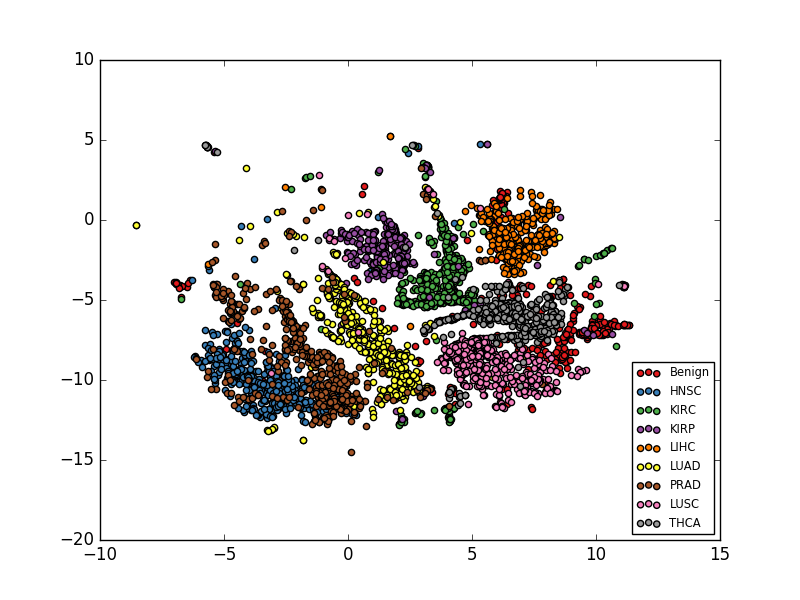
\includegraphics[width=\textwidth]{img/m_r/m_r_sdae_tsne.png}
     \end{subfigure}
        \caption{miRNA-seq and RNA-seq SDAE dGMU model latent space clustered with t-distributed stochastic neighbor embedding (t-SNE).}
        \label{fig:r_m_sdae_tsne}
\end{figure}

\subsubsection{DCF}

\begin{figure}[H]
     \centering
     \begin{subfigure}[b]{0.49\textwidth}
         \centering
         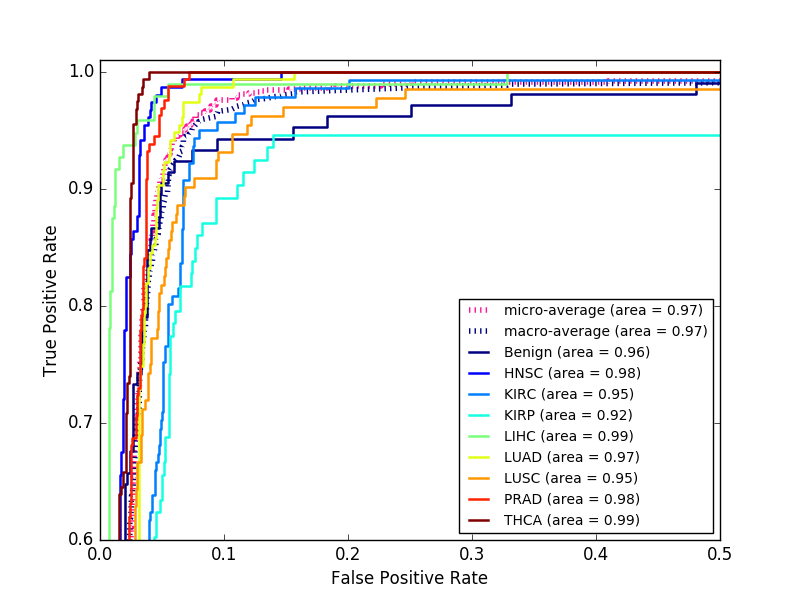
\includegraphics[width=\textwidth]{img/m_r/m_r_dcf_dgmu_roc.png}
         \caption{}
     \end{subfigure}
     \hfill
     \begin{subfigure}[b]{0.49\textwidth}
         \centering
         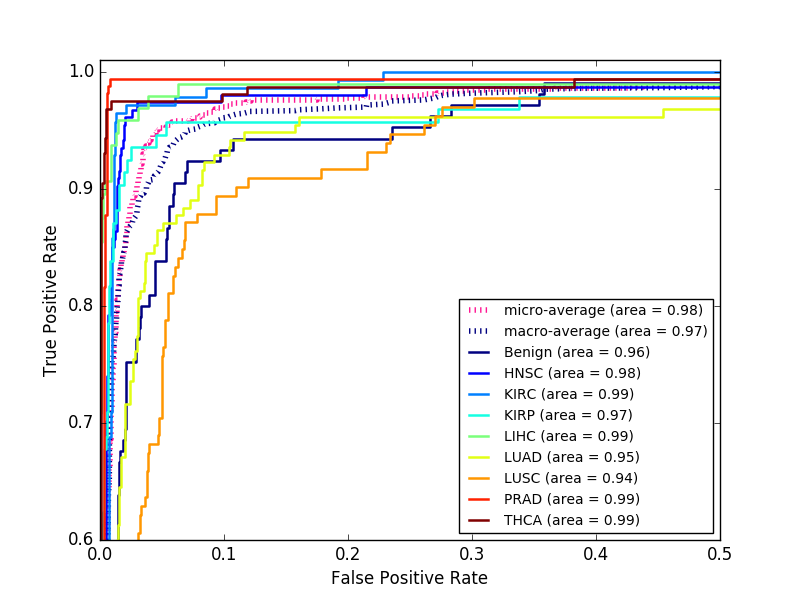
\includegraphics[width=\textwidth]{img/m_r/m_r_dcf_gmu_roc.png}
         \caption{}
     \end{subfigure}
     \hfill
     \begin{subfigure}[b]{0.49\textwidth}
         \centering
         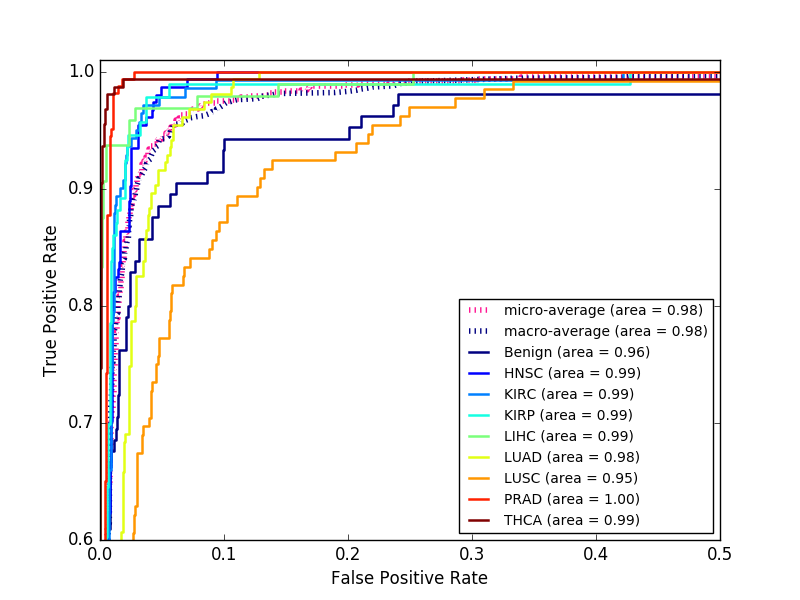
\includegraphics[width=\textwidth]{img/m_r/m_r_dcf_mlp_roc.png}
         \caption{}
     \end{subfigure}
     \begin{subfigure}[b]{0.49\textwidth}
         \centering
         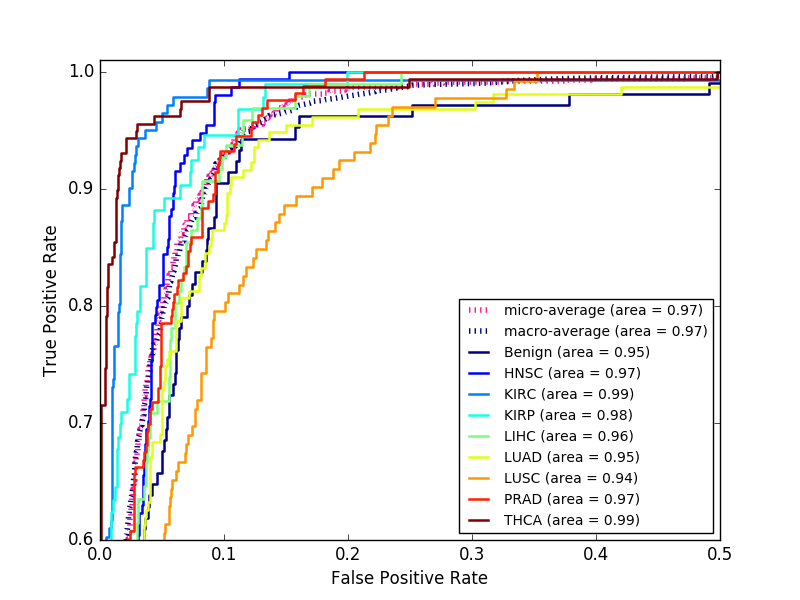
\includegraphics[width=\textwidth]{img/m_r/m_r_dcf_moe_roc.png}
         \caption{}
     \end{subfigure}
        \caption{miRNA-seq and RNA-seq DCF bimodal model ROC plots for a) dGMU b) GMU c) MLP and d) ME.}
        \label{fig:m_r_dcf_roc}
\end{figure}

\begin{table}[H]
   \caption{Summary of classification agreement for miRNA-seq and RNA-seq DCF reduced to 500 features.} 
   \small % text size of table content
   \centering % center the table
   \begin{tabular}{lllll} % alignment of each column data
   \toprule[\heavyrulewidth]\toprule[\heavyrulewidth]
   \textbf{Modality} & \textbf{Accuracy} & \textbf{Precision} & \textbf{Recall} & \textbf{F1-score} \\ 
   \midrule
   \multicolumn{1}{l}{\textbf{Bimodal}} \\
        dGMU & 0.9373 &	0.9385 & 0.9094 & 0.9362\\
        GMU  & 0.9332 &	0.9332 & 0.9332 & 0.9332\\
        MoE  & 0.9106 &	0.9120 & 0.9094 & 0.9107\\
        MLP  & 0.9215 &	0.9208 & 0.9136 & 0.9148\\
        SVM  & 0.8981 &	0.9081 & 0.8922 & 0.9001\\
   \midrule
   \multicolumn{1}{l}{\textbf{miRNA-seq}} \\
        MLP  & 0.8847 &	0.8881 & 0.8815 & 0.8848\\
        SVM  & 0.8739 &	0.8806 & 0.8690 & 0.8748\\
   \midrule
   \multicolumn{1}{l}{\textbf{RNA-seq}}  \\
        MLP  & 0.9023 &	0.9024 & 0.8940 & 0.8982\\
        SVM  & 0.9068 &	0.9116 & 0.9006 & 0.9061\\
   \bottomrule[\heavyrulewidth] 
   \end{tabular}
   \label{table:m_r_dcf_exp41}
\end{table}

\begin{figure}[H]
     \centering
     \begin{subfigure}[b]{\textwidth}
         \centering
         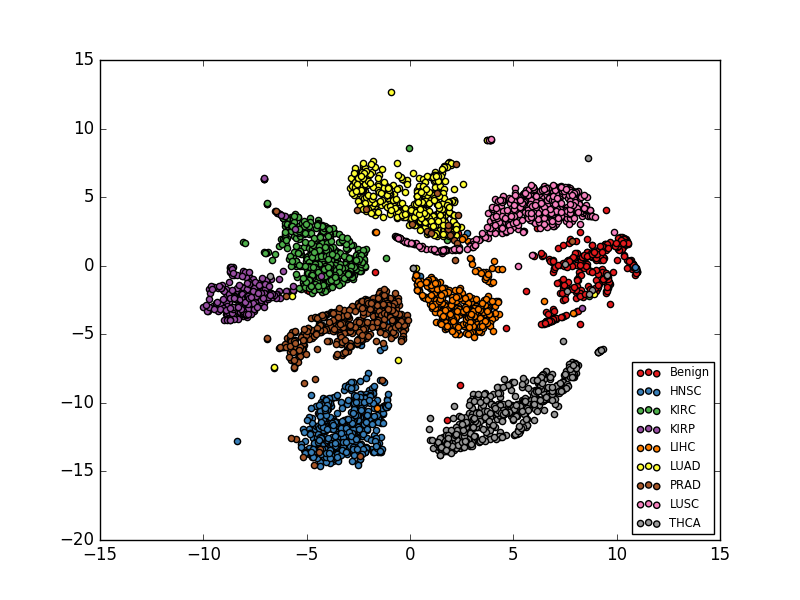
\includegraphics[width=\textwidth]{img/m_r/m_r_dcf_tsne.png}
     \end{subfigure}
        \caption{miRNA-seq and RNA-seq DCF dGMU model latent space clustered with t-distributed stochastic neighbor embedding (t-SNE).}
        \label{fig:r_m_dcf_tsne}
\end{figure}

\subsubsection{DE}

\begin{figure}[H]
     \centering
     \begin{subfigure}[b]{0.49\textwidth}
         \centering
         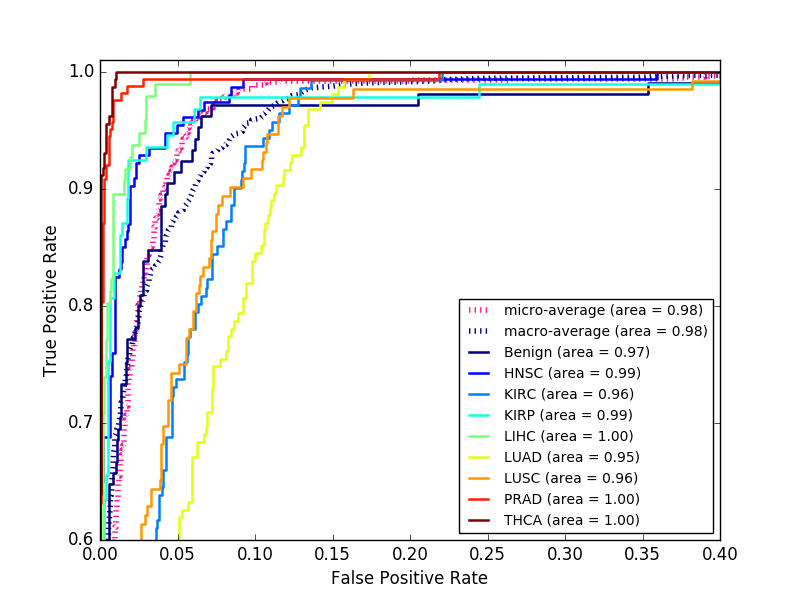
\includegraphics[width=\textwidth]{img/m_r/de_r_m_dgmu_roc.png}
         \caption{}
     \end{subfigure}
     \hfill
     \begin{subfigure}[b]{0.49\textwidth}
         \centering
         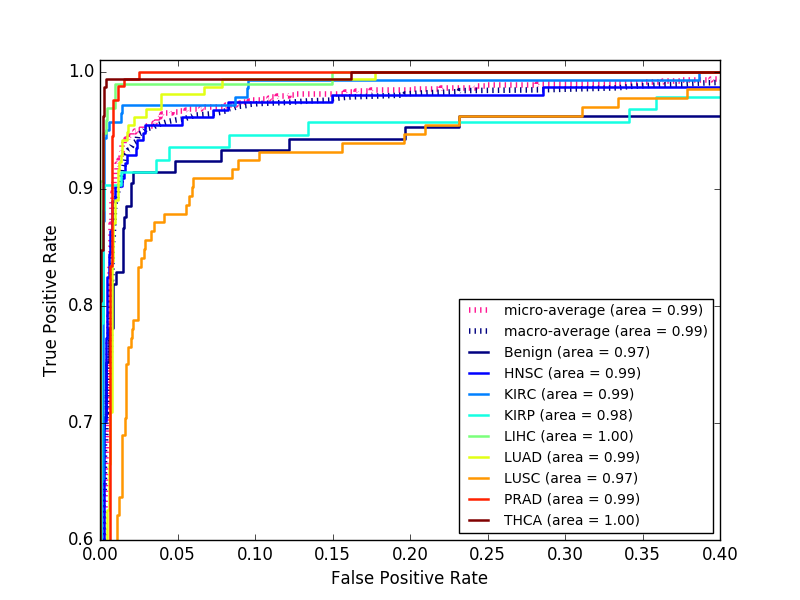
\includegraphics[width=\textwidth]{img/m_r/de_r_m_gmu_roc.png}
         \caption{}
     \end{subfigure}
     \hfill
     \begin{subfigure}[b]{0.49\textwidth}
         \centering
         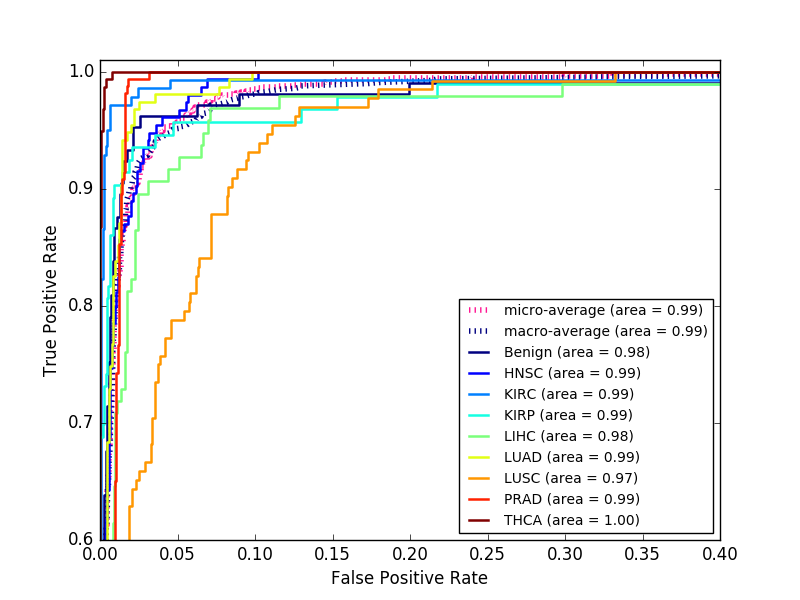
\includegraphics[width=\textwidth]{img/m_r/de_r_m_mlp_roc.png}
         \caption{}
     \end{subfigure}
     \begin{subfigure}[b]{0.49\textwidth}
         \centering
         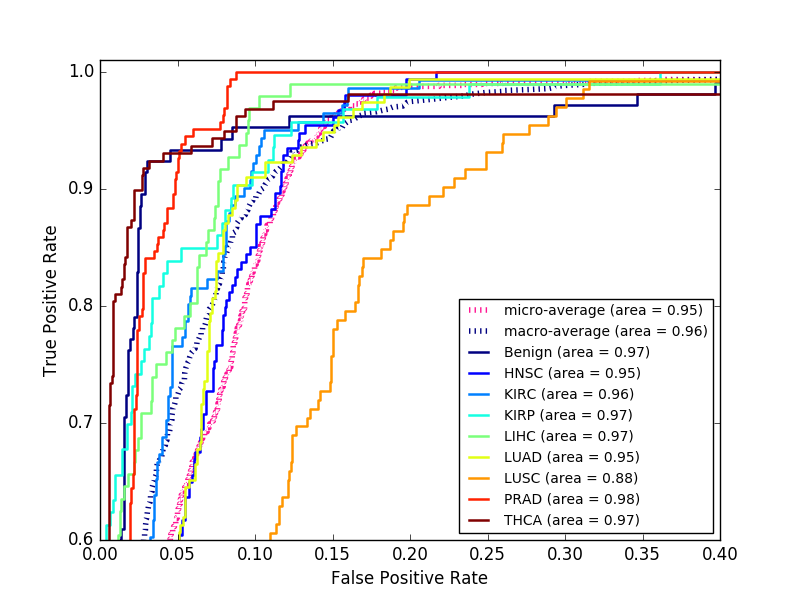
\includegraphics[width=\textwidth]{img/m_r/de_r_m_moe_roc.png}
         \caption{}
     \end{subfigure}
        \caption{miRNA-seq and RNA-seq DE bimodal model ROC plots for a) dGMU b) GMU c) MLP and d) ME.}
        \label{fig:m_r_de_roc}
\end{figure}

\begin{figure}[H]
     \centering
     \begin{subfigure}[b]{\textwidth}
         \centering
         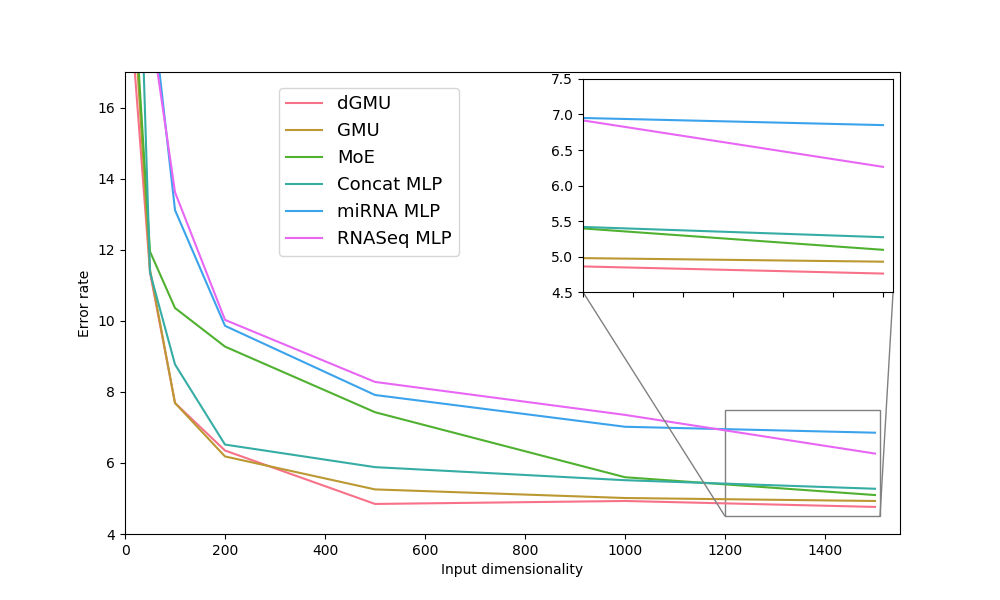
\includegraphics[width=\textwidth]{img/m_r/exp42.png}
     \end{subfigure}
        \caption{miRNA-seq and RNA-seq DE model error rates as a function of input dimensionality.}
        \label{fig:m_r_de_exp42}
\end{figure}

\begin{table}[H]
   \caption{Summary of classification agreement for miRNA-seq and RNA-seq DE reduced to 500 features.} 
   \label{tab:example_multicolumn}
   \small % text size of table content
   \centering % center the table
   \begin{tabular}{lllll} % alignment of each column data
   \toprule[\heavyrulewidth]\toprule[\heavyrulewidth]
   \textbf{Modality} & \textbf{Accuracy} & \textbf{Precision} & \textbf{Recall} & \textbf{F1-score} \\ 
   \midrule
   \multicolumn{1}{l}{\textbf{Bimodal}} \\
        dGMU & 0.9615 & 0.9533 & 0.9496 & 0.9514\\
        GMU  & 0.9475 & 0.9475 & 0.9475 & 0.9475\\
        MoE   & 0.9257 & 0.9327 & 0.9279 & 0.9298\\
        MLP  & 0.9412 & 0.9412 & 0.9401 & 0.9407\\
        SVM  & 0.9257 & 0.9238 & 0.9216 & 0.9227\\
   \midrule
   \multicolumn{1}{l}{\textbf{miRNA-seq}} \\
        MLP  & 0.9209 &	0.9158 & 0.9181 & 0.9215\\
        SVM  & 0.9150 &	0.9158 & 0.9112 & 0.9135\\
   \midrule
   \multicolumn{1}{l}{\textbf{RNA-seq}}  \\
        MLP  & 0.9172 &	0.9192 & 0.9135 & 0.9163\\
        SVM  & 0.9175 &	0.9158 & 0.9125 & 0.9141\\
   \bottomrule[\heavyrulewidth] 
   \end{tabular}
   \label{table:m_r_de_exp41}
\end{table}

\begin{figure}[H]
     \centering
     \begin{subfigure}[b]{\textwidth}
         \centering
         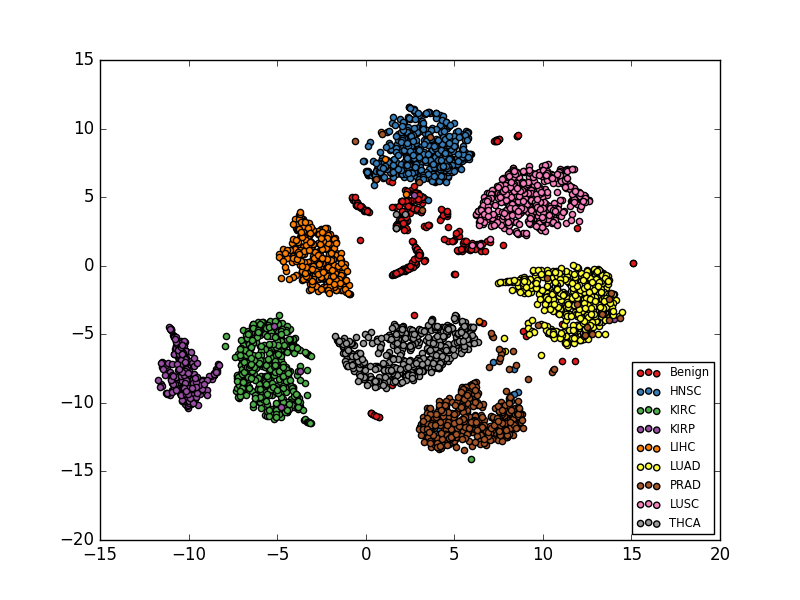
\includegraphics[width=\textwidth]{img/m_r/r_m_de_tsne.png}
         \caption{}
     \end{subfigure}
        \caption{miRNA-seq and RNA-seq DE dGMU model latent space clustered with t-distributed stochastic neighbor embedding (t-SNE).}
        \label{fig:r_m_de_tsne}
\end{figure}

%%%%%%%%%%%%%%%%%%%%%%%%%%%%%%%%%%%%%%%%%%%%%%%%%%%%%%%%%%%%%%%%%%%%%%%%%%%%%%%%%%
%c + R
%%%%%%%%%%%%%%%%%%%%%%%%%%%%%%%%%%%%%%%%%%%%%%%%%%%%%%%%%%%%%%%%%%%%%%%%%%%%%%%%%%

\subsection{CNV + RNA-seq}\label{sub:c_r_results}

\subsubsection{SDAE}

\begin{figure}[H]
     \centering
     \begin{subfigure}[b]{0.49\textwidth}
         \centering
         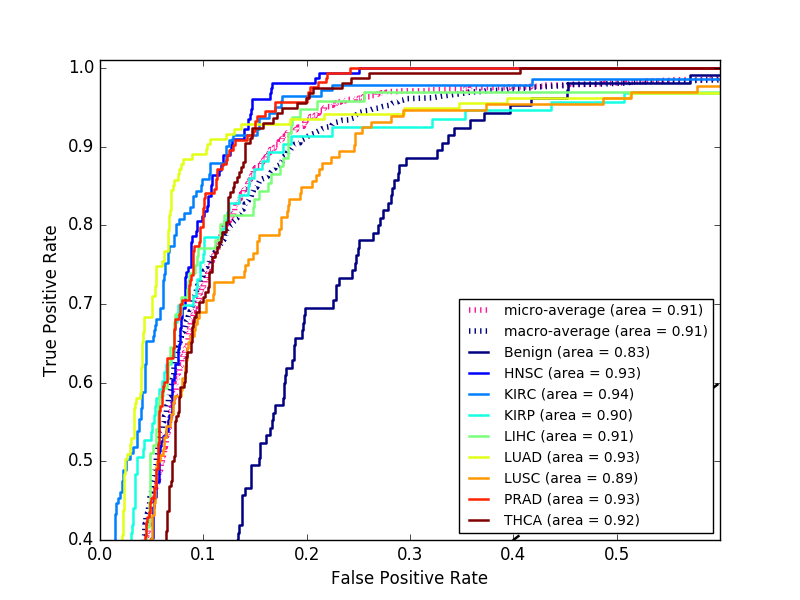
\includegraphics[width=\textwidth]{img/c_r/c_r_sdae_dgmu_roc.png}
         \caption{}
     \end{subfigure}
     \hfill
     \begin{subfigure}[b]{0.49\textwidth}
         \centering
         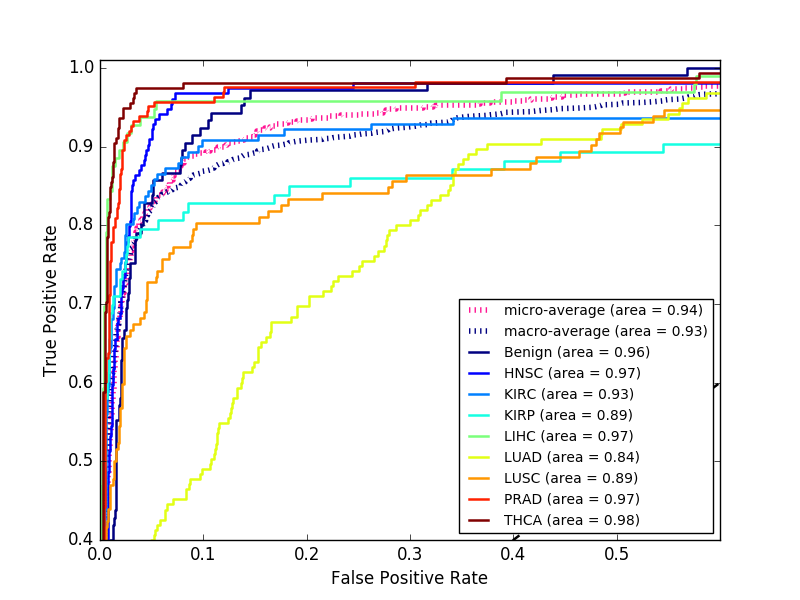
\includegraphics[width=\textwidth]{img/c_r/c_r_sdae_gmu_roc.png}
         \caption{}
     \end{subfigure}
     \hfill
     \begin{subfigure}[b]{0.49\textwidth}
         \centering
         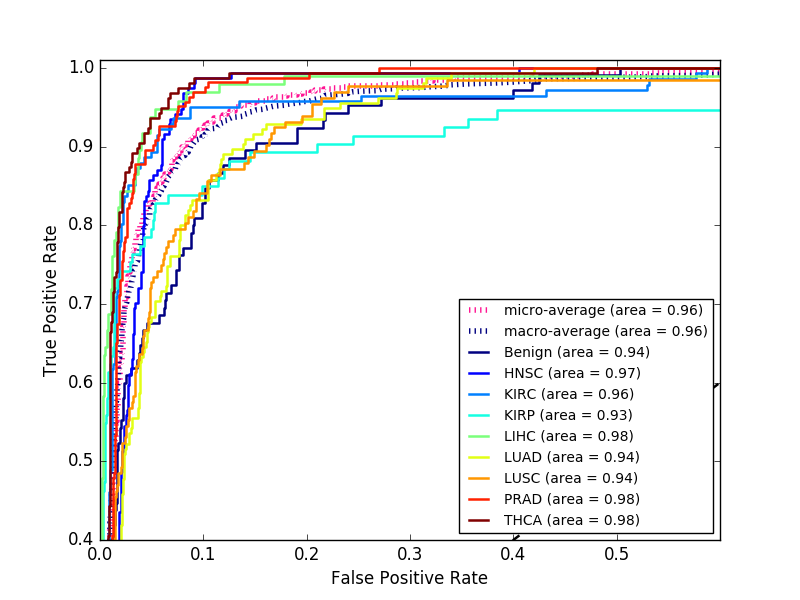
\includegraphics[width=\textwidth]{img/c_r/c_r_sdae_mlp_roc.png}
         \caption{}
     \end{subfigure}
     \begin{subfigure}[b]{0.49\textwidth}
         \centering
         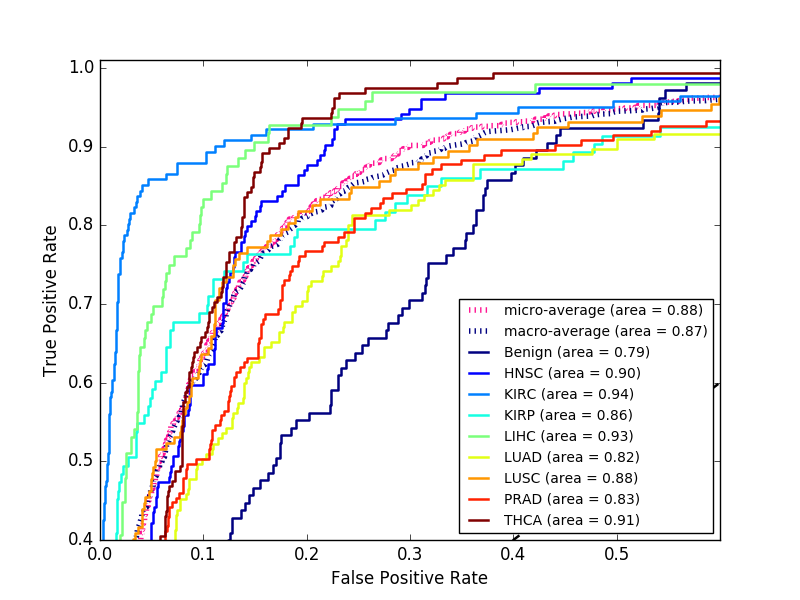
\includegraphics[width=\textwidth]{img/c_r/c_r_sdae_moe_roc.png}
         \caption{}
     \end{subfigure}
        \caption{CNV and RNA-seq SDAE bimodal model ROC plots for a) dGMU b) GMU c) MLP and d) ME.}
        \label{fig:c_r_sdae_roc}
\end{figure}

\begin{table}[H]
   \caption{Summary of classification agreement for CNV and RNA-seq SDAE reduced to 500 features.} 
   \small % text size of table content
   \centering % center the table
   \begin{tabular}{lllll} % alignment of each column data
   \toprule[\heavyrulewidth]\toprule[\heavyrulewidth]
   \textbf{Modality} & \textbf{Accuracy} & \textbf{Precision} & \textbf{Recall} & \textbf{F1-score} \\ 
   \midrule
   \multicolumn{1}{l}{\textbf{Bimodal}} \\
        dGMU & 0.8764 &	0.8739 & 0.8749 & 0.8737\\
        GMU  & 0.8722 &	0.8700 & 0.8661 & 0.8675\\
        MoE  & 0.7611 &	0.7617 & 0.7566 & 0.7556\\
        MLP  & 0.8622 &	0.8613 & 0.8542 & 0.8570\\
        SVM  & 0.8605 &	0.8567 & 0.8542 & 0.8550\\
   \midrule
   \multicolumn{1}{l}{\textbf{CNV}} \\
        MLP  & 0.7586 &	0.7622 & 0.7534 & 0.7526\\
        SVM  & 0.7343 &	0.7459 & 0.7275 & 0.7321\\
   \midrule
   \multicolumn{1}{l}{\textbf{RNA-seq}}  \\
        MLP  & 0.8530 &	0.8560 & 0.8425 & 0.8477\\
        SVM  & 0.8429 &	0.8388 & 0.8347 & 0.8362\\
   \bottomrule[\heavyrulewidth] 
   \end{tabular}
   \label{table:c_r_sdae_exp41}
\end{table}

\begin{figure}[H]
     \centering
     \begin{subfigure}[b]{\textwidth}
         \centering
         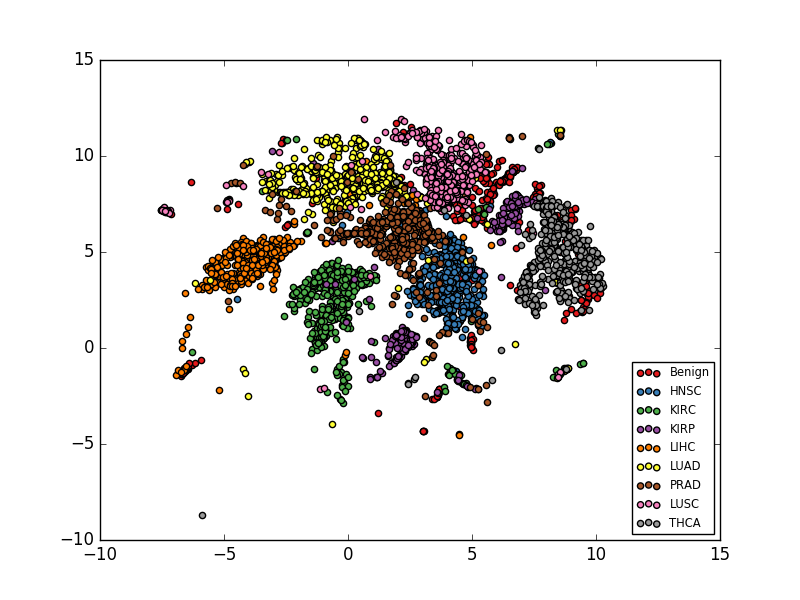
\includegraphics[width=\textwidth]{img/c_r/c_r_sdae_tsne.png}
     \end{subfigure}
        \caption{CNV and RNA-seq SDAE dGMU model latent space clustered with t-distributed stochastic neighbor embedding (t-SNE).}
        \label{fig:c_r_sdae_tsne}
\end{figure}

\subsubsection{DCF}

\begin{figure}[H]
     \centering
     \begin{subfigure}[b]{0.49\textwidth}
         \centering
         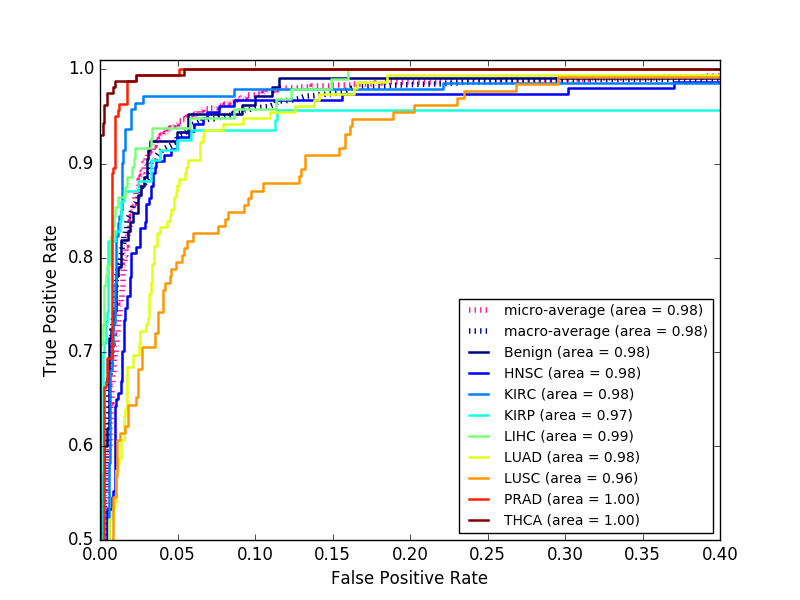
\includegraphics[width=\textwidth]{img/c_r/c_r_dcf_dgmu_roc.png}
         \caption{}
     \end{subfigure}
     \hfill
     \begin{subfigure}[b]{0.49\textwidth}
         \centering
         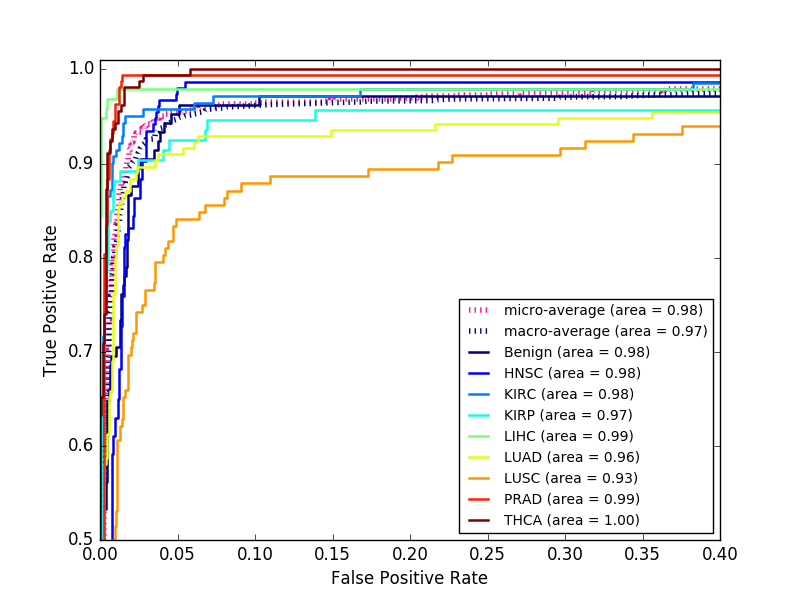
\includegraphics[width=\textwidth]{img/c_r/c_r_dcf_gmu_roc.png}
         \caption{}
     \end{subfigure}
     \hfill
     \begin{subfigure}[b]{0.49\textwidth}
         \centering
         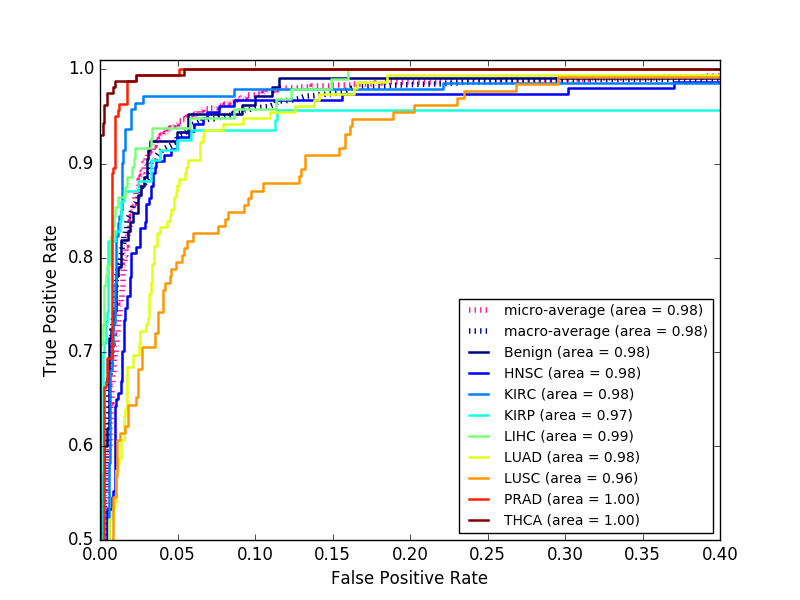
\includegraphics[width=\textwidth]{img/c_r/c_r_dcf_mlp_roc.png}
         \caption{}
     \end{subfigure}
     \begin{subfigure}[b]{0.49\textwidth}
         \centering
         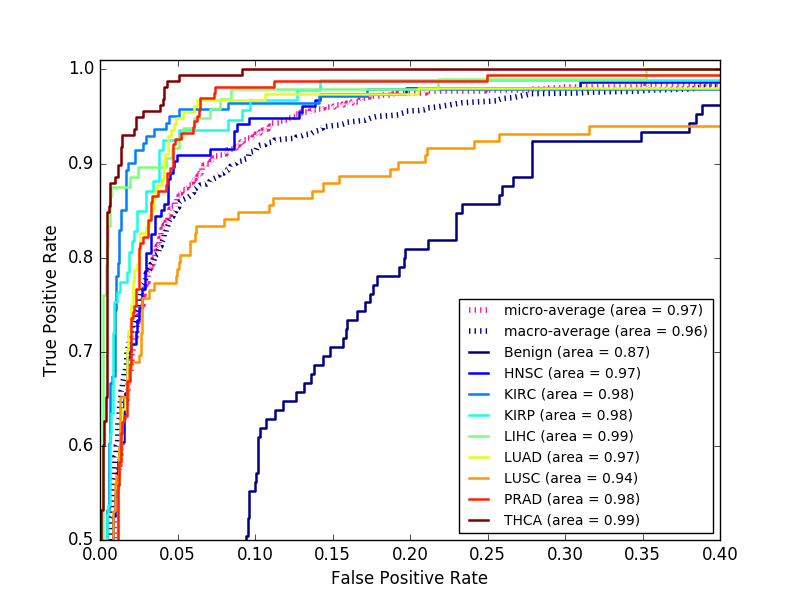
\includegraphics[width=\textwidth]{img/c_r/c_r_dcf_moe_roc.png}
         \caption{}
     \end{subfigure}
        \caption{CNV and RNA-seq DCF bimodal model ROC plots for a) dGMU b) GMU c) MLP and d) ME.}
        \label{fig:c_r_dcf_roc}
\end{figure}

\begin{figure}[H]
     \centering
     \begin{subfigure}[b]{\textwidth}
         \centering
         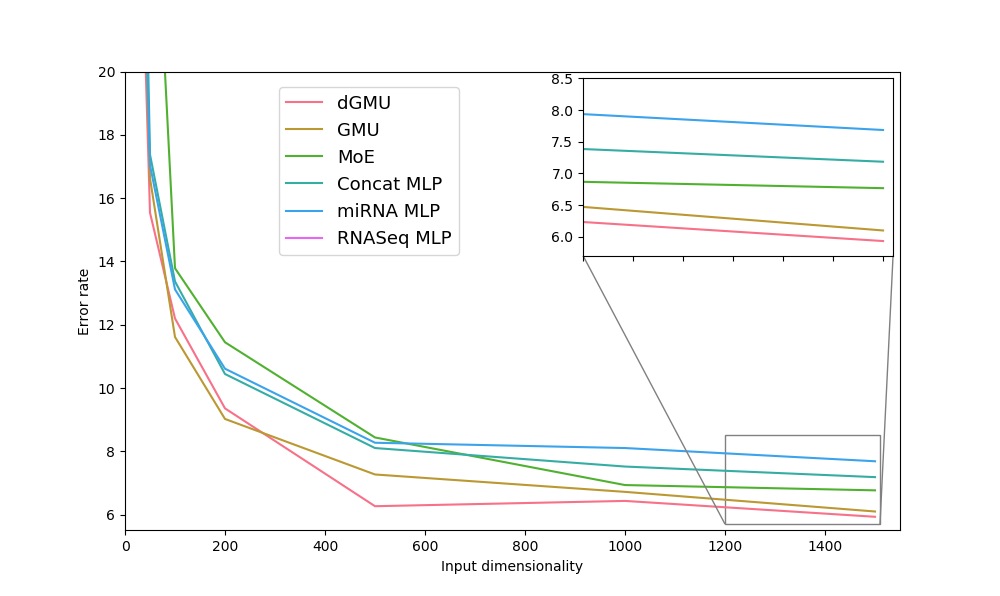
\includegraphics[width=\textwidth]{img/c_r/exp82.png}
     \end{subfigure}
        \caption{CNV and RNA-seq DE model error rates as a function of input dimensionality.}
        \label{fig:c_r_dcf_exp82}
\end{figure}

\begin{table}[H]
   \caption{Summary of classification agreement for CNV and RNA-seq DCF reduced to 500 features.} 
   \small % text size of table content
   \centering % center the table
   \begin{tabular}{lllll} % alignment of each column data
   \toprule[\heavyrulewidth]\toprule[\heavyrulewidth]
   \textbf{Modality} & \textbf{Accuracy} & \textbf{Precision} & \textbf{Recall} & \textbf{F1-score} \\ 
   \midrule
   \multicolumn{1}{l}{\textbf{Bimodal}} \\
        dGMU & 0.9373 &	0.9373 & 0.9373 & 0.9373\\
        GMU  & 0.9273 &	0.9273 & 0.9273 & 0.9273\\
        MoE  & 0.9156 &	0.9109 & 0.9111 & 0.9109\\
        MLP  & 0.9189 &	0.9199 & 0.9123 & 0.9154\\
        SVM  & 0.9172 &	0.9175 & 0.9150 & 0.9136\\
   \midrule
   \multicolumn{1}{l}{\textbf{CNV}} \\
        MLP  & 0.7468 &	0.7795 & 0.7270 & 0.7200\\
        SVM  & 0.7335 &	0.7460 & 0.7256 & 0.7310\\
   \midrule
   \multicolumn{1}{l}{\textbf{RNA-seq}}  \\
        MLP  & 0.9097 &	0.9118 & 0.9022 & 0.9052\\
        SVM  & 0.9072 &	0.9104 & 0.9045 & 0.9004\\
   \bottomrule[\heavyrulewidth] 
   \end{tabular}
   \label{table:c_r_dcf_exp41}
\end{table}

\begin{figure}[H]
     \centering
     \begin{subfigure}[b]{\textwidth}
         \centering
         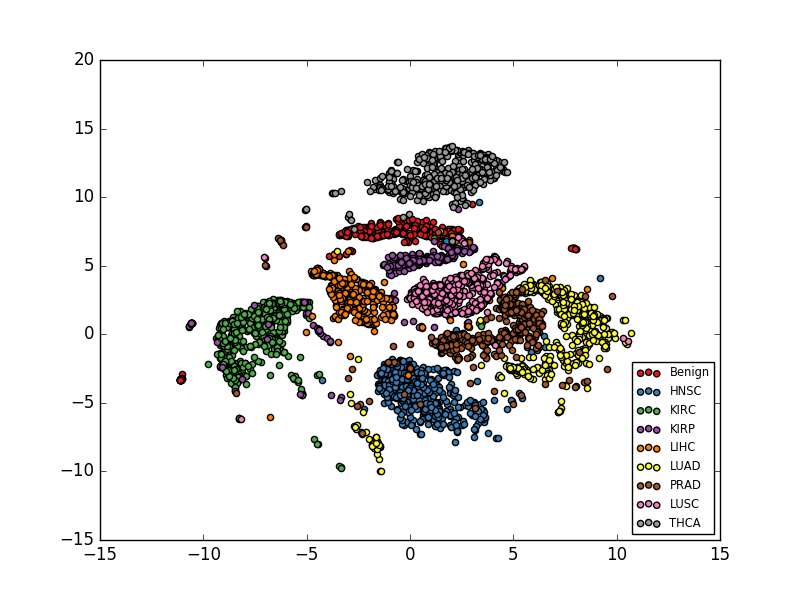
\includegraphics[width=\textwidth]{img/c_r/c_r_dcf_tsne.png}
     \end{subfigure}
        \caption{CNV and RNA-seq DCF dGMU model latent space clustered with t-distributed stochastic neighbor embedding (t-SNE).}
        \label{fig:c_r_dcf_tsne}
\end{figure}

%%%%%%%%%%%%%%%%%%%%%%%%%%%%%%%%%%%%%%%%%%%%%%%%%%%%%%%%%%%%%%%%%%%%%%%%%%%%%%%%%%
%M + S
%%%%%%%%%%%%%%%%%%%%%%%%%%%%%%%%%%%%%%%%%%%%%%%%%%%%%%%%%%%%%%%%%%%%%%%%%%%%%%%%%%

\subsection{miRNA-seq + SNV}\label{sub:m_s_results}

\subsubsection{SDAE}

\begin{figure}[H]
     \centering
     \begin{subfigure}[b]{0.49\textwidth}
         \centering
         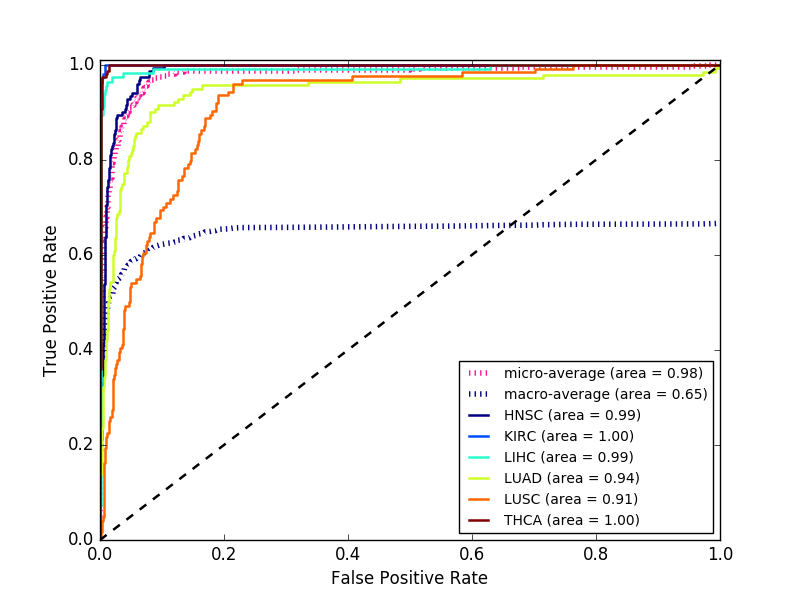
\includegraphics[width=\textwidth]{img/m_s/m_s_sdae_dgmu_roc.png}
         \caption{}
     \end{subfigure}
     \hfill
     \begin{subfigure}[b]{0.49\textwidth}
         \centering
         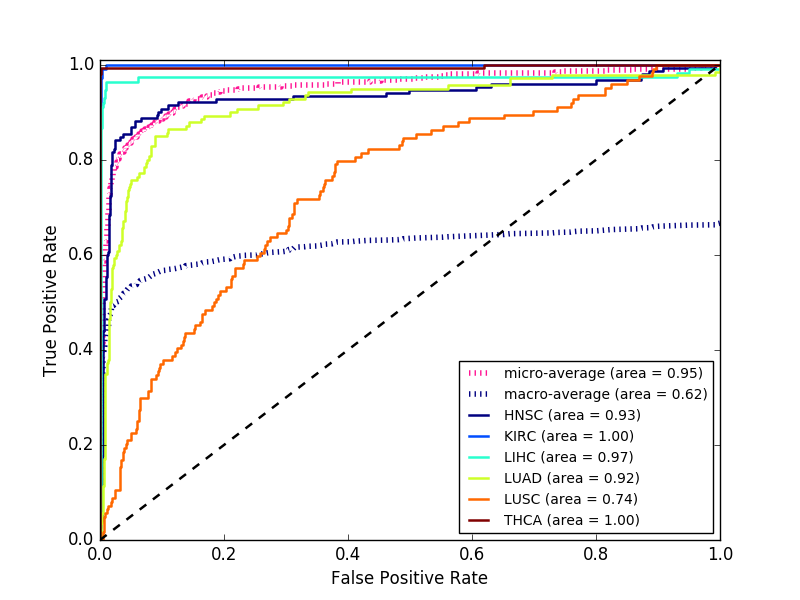
\includegraphics[width=\textwidth]{img/m_s/m_s_sdae_gmu_roc.png}
         \caption{}
     \end{subfigure}
     \hfill
     \begin{subfigure}[b]{0.49\textwidth}
         \centering
         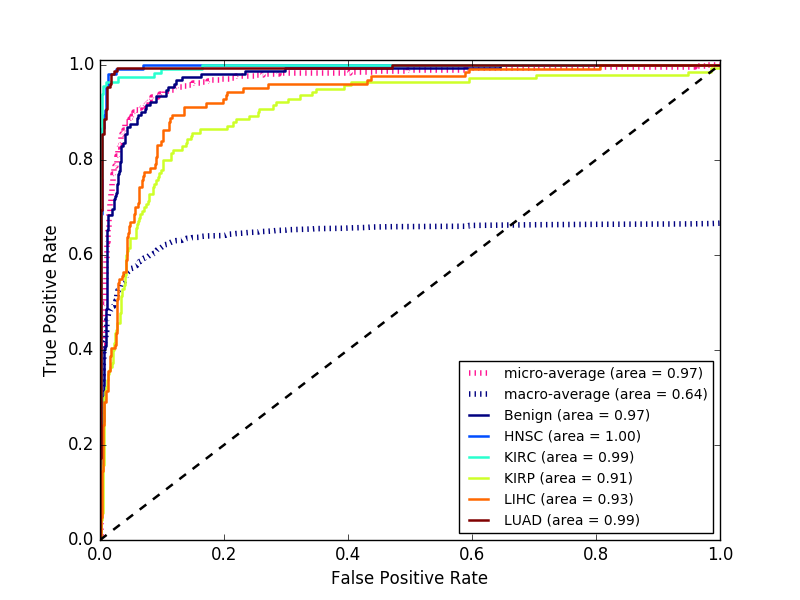
\includegraphics[width=\textwidth]{img/m_s/m_s_sdae_mlp_roc.png}
         \caption{}
     \end{subfigure}
     \begin{subfigure}[b]{0.49\textwidth}
         \centering
         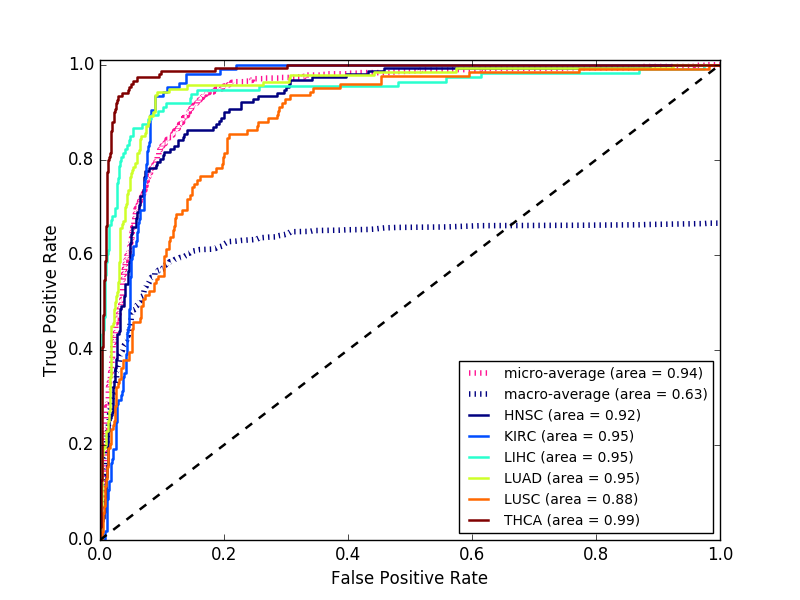
\includegraphics[width=\textwidth]{img/m_s/m_s_sdae_moe_roc.png}
         \caption{}
     \end{subfigure}
        \caption{miRNA-seq and SNV SDAE bimodal model ROC plots for a) dGMU b) GMU c) MLP and d) ME.}
        \label{fig:m_s_sdae_roc}
\end{figure}

\begin{table}[H]
   \caption{Summary of classification agreement for miRNA-seq and SNV SDAE reduced to 500 features.} 
   \small % text size of table content
   \centering % center the table
   \begin{tabular}{lllll} % alignment of each column data
   \toprule[\heavyrulewidth]\toprule[\heavyrulewidth]
   \textbf{Modality} & \textbf{Accuracy} & \textbf{Precision} & \textbf{Recall} & \textbf{F1-score} \\ 
   \midrule
   \multicolumn{1}{l}{\textbf{Bimodal}} \\
        dGMU & 0.9362 & 0.9375 & 0.9372 & 0.9373\\
        GMU  & 0.9260 & 0.9260 & 0.9260 & 0.9260\\
        MoE  & 0.9145 & 0.9199 & 0.9161 & 0.9173\\
        MLP  & 0.9222 & 0.9228 & 0.9227 & 0.9223\\
        SVM  & 0.9171 & 0.9198 & 0.9205 & 0.9199\\
   \midrule
   \multicolumn{1}{l}{\textbf{miRNA-seq}} \\
        MLP  & 0.9120 & 0.9207 & 0.9093 & 0.9113\\
        SVM  & 0.9107 & 0.9148 & 0.9134 & 0.9134\\
   \midrule
   \multicolumn{1}{l}{\textbf{SNV}}  \\
        MLP  & 0.6480 & 0.6454 & 0.6400 & 0.6407\\
        SVM  & 0.6173 & 0.6036 & 0.6013 & 0.6048\\
   \bottomrule[\heavyrulewidth] 
   \end{tabular}
   \label{table:c_r_sdae_summary}
\end{table}

\begin{figure}[H]
     \centering
     \begin{subfigure}[b]{\textwidth}
         \centering
         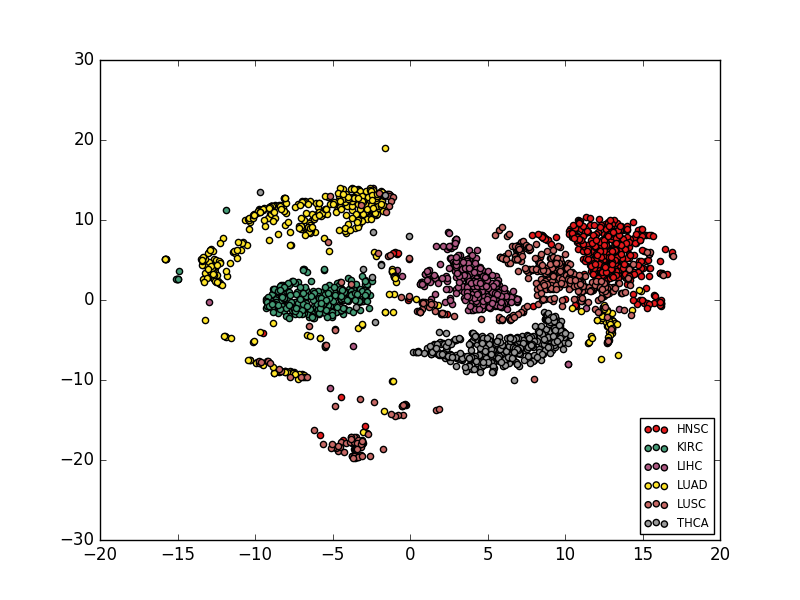
\includegraphics[width=\textwidth]{img/m_s/m_s_sdae_tsne.png}
     \end{subfigure}
        \caption{miRNA-seq and SNV SDAE dGMU model latent space clustered with t-distributed stochastic neighbor embedding (t-SNE).}
        \label{fig:m_s_sdae_tsne}
\end{figure}

\subsubsection{DCF}

\begin{figure}[H]
     \centering
     \begin{subfigure}[b]{0.49\textwidth}
         \centering
         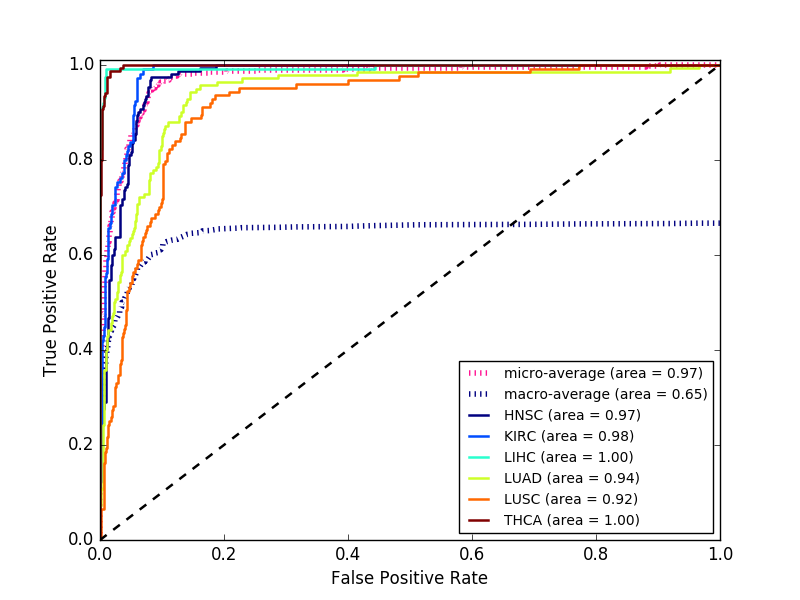
\includegraphics[width=\textwidth]{img/m_s/m_s_dcf_dgmu_roc.png}
         \caption{}
     \end{subfigure}
     \hfill
     \begin{subfigure}[b]{0.49\textwidth}
         \centering
         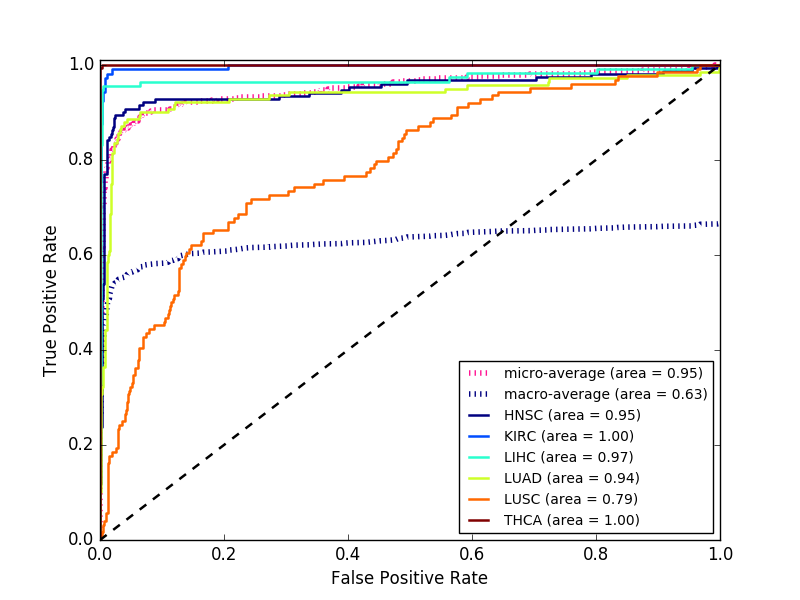
\includegraphics[width=\textwidth]{img/m_s/m_s_dcf_gmu_roc.png}
         \caption{}
     \end{subfigure}
     \hfill
     \begin{subfigure}[b]{0.49\textwidth}
         \centering
         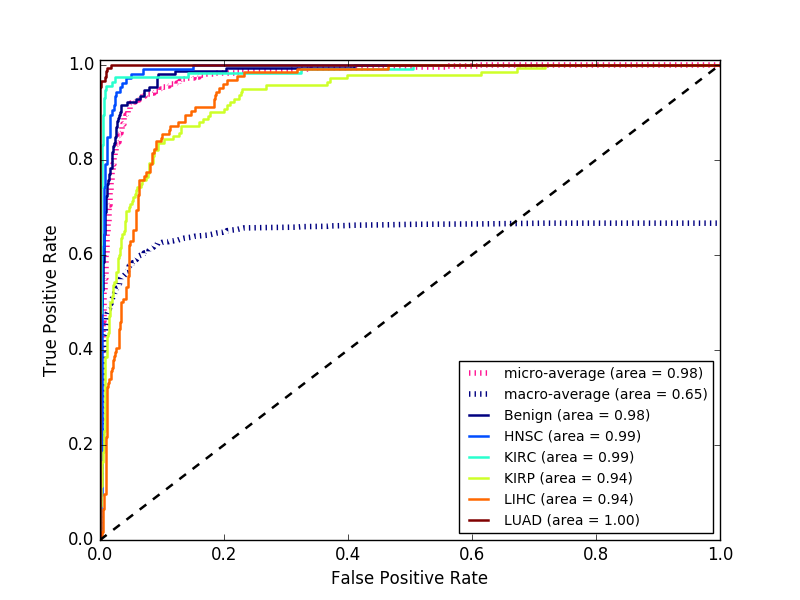
\includegraphics[width=\textwidth]{img/m_s/m_s_dcf_mlp_roc.png}
         \caption{}
     \end{subfigure}
     \begin{subfigure}[b]{0.49\textwidth}
         \centering
         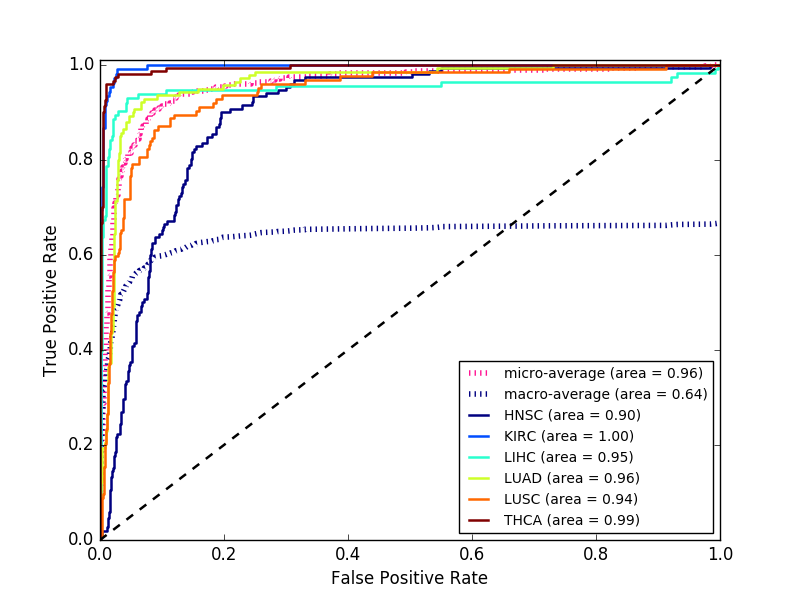
\includegraphics[width=\textwidth]{img/m_s/m_s_dcf_moe_roc.png}
         \caption{}
     \end{subfigure}
        \caption{miRNA-seq and SNV DCF bimodal model ROC plots for a) dGMU b) GMU c) MLP and d) ME.}
        \label{fig:m_s_dcf_roc}
\end{figure}

\begin{figure}[H]
     \centering
     \begin{subfigure}[b]{\textwidth}
         \centering
         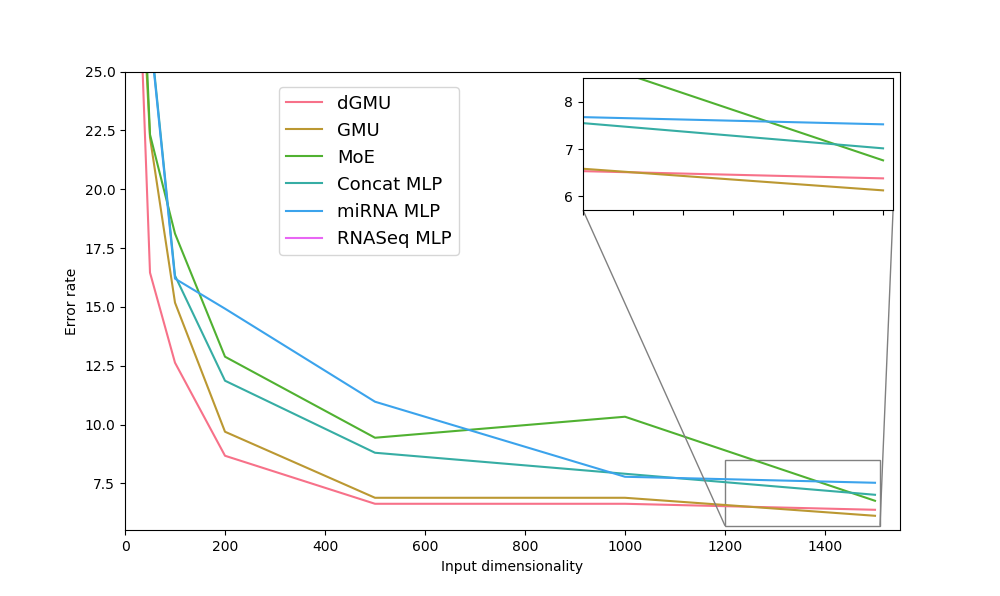
\includegraphics[width=\textwidth]{img/m_s/exp92.png}
     \end{subfigure}
        \caption{miRNA-seq and SNV DCF model error rates as a function of input dimensionality.}
        \label{fig:m_s_dcf_exp92}
\end{figure}

\begin{table}[H]
   \caption{Summary of classification agreement for miRNA-seq and SNV DCF reduced to 500 features.} 
   \small % text size of table content
   \centering % center the table
   \begin{tabular}{lllll} % alignment of each column data
   \toprule[\heavyrulewidth]\toprule[\heavyrulewidth]
   \textbf{Modality} & \textbf{Accuracy} & \textbf{Precision} & \textbf{Recall} & \textbf{F1-score} \\ 
   \midrule
   \multicolumn{1}{l}{\textbf{Bimodal}} \\
        dGMU & 0.9337 & 0.9358 & 0.9336 & 0.9334\\
        GMU  & 0.9324 & 0.9324 & 0.9324 & 0.9324\\
        MoE  & 0.9056 & 0.9067 & 0.9073 & 0.9070\\
        MLP  & 0.9120 & 0.9171 & 0.9154 & 0.9150\\
        SVM  & 0.8903 & 0.8921 & 0.8929 & 0.8924\\
   \midrule
   \multicolumn{1}{l}{\textbf{miRNA-seq}} \\
        MLP  & 0.9056 & 0.9073 & 0.9084 & 0.9077\\
        SVM  & 0.8980 & 0.8995 & 0.9006 & 0.8999\\
   \midrule
   \multicolumn{1}{l}{\textbf{SNV}}  \\
        MLP  & 0.5523 & 0.5834 & 0.5465 & 0.5512\\
        SVM  & 0.5599 & 0.5541 & 0.5561 & 0.5425\\
   \bottomrule[\heavyrulewidth] 
   \end{tabular}
   \label{table:m_s_dcf_summary}
\end{table}

\begin{figure}[H]
     \centering
     \begin{subfigure}[b]{\textwidth}
         \centering
         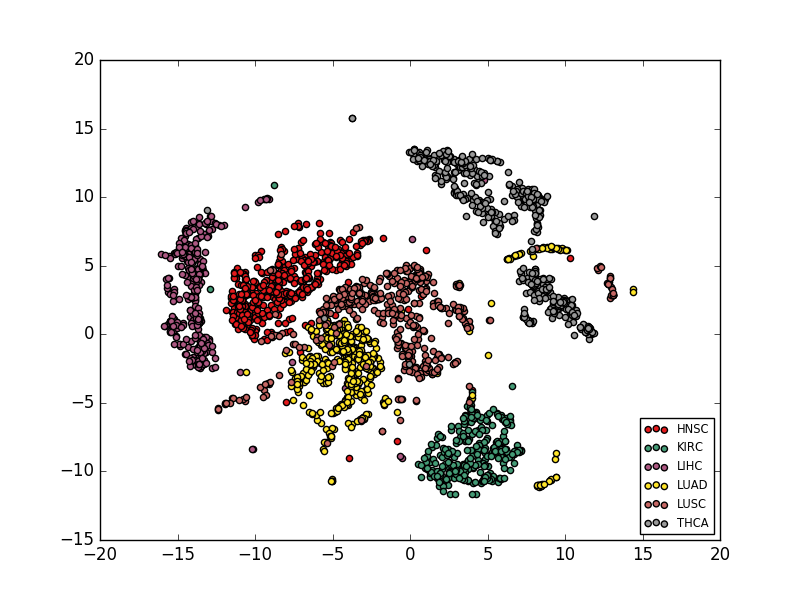
\includegraphics[width=\textwidth]{img/m_s/m_s_dcf_tsne.png}
     \end{subfigure}
        \caption{miRNA-seq and SNV DCF dGMU model latent space clustered with t-distributed stochastic neighbor embedding (t-SNE).}
        \label{fig:m_s_dcf_tsne}
\end{figure}